\documentclass{sig-alternate} 

\usepackage{times}
\usepackage{mathtools}
\usepackage{amsmath}
\usepackage{comment}
\usepackage{graphicx}
\usepackage{color}
\usepackage{amsfonts}
\newcommand{\pluseq}{\mathrel{+}=}

\usepackage{mathptmx} % This is Times font
\newcommand{\IGNORE}[1]{}
\usepackage{fancyhdr}
\usepackage[normalem]{ulem}
\usepackage[hyphens]{url}
\usepackage{hyperref}

%%%%%%%%%%%---SETME-----%%%%%%%%%%%%%
\newcommand{\hpcasubmissionnumber}{NaN}
%%%%%%%%%%%%%%%%%%%%%%%%%%%%%%%%%%%%

\fancypagestyle{firstpage}{
  \fancyhf{}
\setlength{\headheight}{50pt}
\renewcommand{\headrulewidth}{0pt}
  \fancyhead[C]{\normalsize{ISCA 2016 Submission
      \textbf{\#\hpcasubmissionnumber} \\ Confidential Draft: DO NOT DISTRIBUTE}} 
  \pagenumbering{arabic}
}  

%\renewcommand{\baselinestretch}{0.942}

%% general operators
\newcommand{\card}[1]{\left\vert{#1}\right\vert}
\newcommand{\set}[1]{\left\{{#1}\right\}}

% model parameters
\newcommand{\sampletime}{T_{sample}}
\newcommand{\replicatime}[1]{{T(#1)}}
\newcommand{\epochtime}[1]{{T_{epoch}(#1)}}
\newcommand{\layertime}[1]{{T_{layer}(#1)}}
\newcommand{\layerepoch}[2]{{T_{epoch}(#1,#2)}}
\newcommand{\timeforwardone}[1]{{T_{F}(#1)}}
\newcommand{\timebackwardone}[1]{{T_{B}(#1)}}
\newcommand{\timeweightupdate}[1]{{T_{W}(#1)}}
\newcommand{\timeforwardtwo}[2]{{T_{F}(#1,#2)}}
\newcommand{\timebackwardtwo}[2]{{T_{B}(#1,#2)}}
\newcommand{\timeweightupdatetwo}[2]{{T_{W}(#1,#2)}}

\newcommand{\compward}[2]{{P(#1,#2)}}
\newcommand{\compforward}[2]{{P_{F}(#1,#2)}}
\newcommand{\compforwardfull}[3]{{P_{F}(#1,#2,#3)}}
\newcommand{\compforwardentire}[4]{{P_{F}(#1,#2,#3,#4)}}
\newcommand{\compforwardlayer}[2]{{TP_{F}(#1,#2)}}
\newcommand{\compforwardsample}[1]{{P^{'}_{F}(#1)}}
\newcommand{\commforward}[2]{{M_{F}(#1,#2)}}
\newcommand{\commforwardfull}[3]{{M_{F}(#1,#2,#3)}}
\newcommand{\commforwardentire}[4]{{M_{F}(#1,#2,#3,#4)}}
\newcommand{\commforwardlayer}[2]{{TM_{F}(#1,#2)}}

\newcommand{\compone}[2]{{P_{i}(#1,#2)}}
\newcommand{\compall}[3]{{P_{i}(#1,#2,#3)}}
\newcommand{\commall}[3]{{M_{i}(#1,#2,#3)}}

\newcommand{\commward}[2]{{M(#1,#2)}}
\newcommand{\compbackward}[2]{{P_{B}(#1,#2)}}
\newcommand{\compbackwardfull}[3]{{P_{B}(#1,#2,#3)}}
\newcommand{\compbackwardentire}[4]{{P_{B}(#1,#2,#3,#4)}}
\newcommand{\compbackwardlayer}[2]{{TP_{B}(#1,#2)}}
\newcommand{\commbackward}[2]{{M_{B}(#1,#2)}}
\newcommand{\commbackwardfull}[3]{{M_{B}(#1,#2,#3)}}
\newcommand{\commbackwardentire}[4]{{M_{B}(#1,#2,#3,#4)}}
\newcommand{\commbackwardlayer}[2]{{TM_{B}(#1,#2)}}

\newcommand{\compweightupdate}[2]{{P_{W}(#1,#2)}}
\newcommand{\compweightupdateentire}[4]{{P_{W}(#1,#2,#3,#4)}}
\newcommand{\commweightupdate}[2]{{M_{W}(#1,#2)}}
\newcommand{\weightvector}[2]{\hat{w}_{#1}(#2)}
\newcommand{\weightnumber}[2]{W_{#1}(#2)}
\newcommand{\weightnumberprime}[2]{W^{'}_{#1}(#2)}

\newcommand{\remoteall}[3]{{R_{i}(#1,#2,#3)}}
\newcommand{\remoteforward}[2]{{R_{F}(#1,#2)}}
\newcommand{\remoteforwardfull}[3]{{R_{F}(#1,#2,#3)}}
\newcommand{\remoteforwardentire}[4]{{R_{B}(#1,#2,#3,#4)}}
\newcommand{\remotebackward}[2]{{R_{B}(#1,#2)}}
\newcommand{\remotebackwardfull}[3]{{R_{B}(#1,#2,#3)}}
\newcommand{\remotebackwardentire}[4]{{R_{B}(#1,#2,#3,#4)}}

\newcommand{\degrees}[1]{{N_{p}(#1)}}
\newcommand{\activation}[2]{{N_{neuron}(#1,#2)}}
\newcommand{\weights}{N_{W}}
\newcommand{\reads}{N_{read}}
\newcommand{\paraserver}{P_{S}}
\newcommand{\replicas}{R_{A}}
\newcommand{\workers}{W_{O}}
\newcommand{\machines}{M_{A}}
\newcommand{\samples}{N_{S}}
\newcommand{\segments}[1]{{Seg(#1)}}


%constants
\newcommand{\constmuladd}{C_{MulAdd}}
\newcommand{\constactivation}{C_{Act}}
\newcommand{\constderivative}{C_{Der}}
\newcommand{\consterror}{C_{Err}}
\newcommand{\constweight}{C_{Weight}}
\newcommand{\constweightbatch}{CB_{Weight}}

\newcommand{\netlatency}{C_{NCost}}
\newcommand{\netlatencyfull}[1]{{C_{NCost}(#1)}}
\newcommand{\netbandwidth}{C_{NBandwidth}}
\newcommand{\netbandwidthfull}[1]{{C_{NBandwidth}(#1)}}
\newcommand{\bitsperactivation}{C_{BitsPerAct}}
\newcommand{\bitsperweight}{C_{BitsPerWeight}}
\newcommand{\segweights}[4]{{D_{Weight}(#1,#2,#3,#4)}}
\newcommand{\layerweights}[1]{{D_{Weight}(#1)}}
\newcommand{\interference}[1]{{C_{I}(#1)}}

%\newcommand{\replicatimeall}{T(Replica)}
%\newcommand{\netlatency}[1]{{C_{NCost}(#1)}}
%\newcommand{\dataforward}[2]{{D_{F}(#1,#2)}}

\begin{document}

%\title{Efficient Sparse Data Computations for Deep Learning}
\title{Accelerating Deep Learning via Architectural Support for Efficient Sparse Data Computation and Storage}
%\author{Anonymous}
\date{}
\maketitle
\thispagestyle{firstpage}
\pagestyle{plain}

%\setlength{\belowdisplayskip}{5pt} \setlength{\belowdisplayshortskip}{5pt}
%\setlength{\abovedisplayskip}{5pt} \setlength{\abovedisplayshortskip}{5pt}

\begin{abstract}
Deep learning has recently emerged as an important machine learning approach, with big deep neural networks (DNN) models trained on vast amounts of data demonstrating state-of-the-art accuracy on important yet challenging artificial intelligence tasks, such as image and speech recognition.  However, training big DNN models using large training data is both compute and memory intensive,  making distributed training on a cluster of server machines, leveraging the aggregate system resources, the standard approach.

This paper proposes hardware techniques for improving system performance and scalability for DNN training workloads by exploiting the sparse nature of computation to reduce the compute and memory requirements.  Our techniques improve training efficiency by avoiding resource utilization on sparse data values (i.e., zeroes) which do not impact training quality. Our design is transparent to software, enabling existing codes to enjoy a performance boost without modifications. 

Simulation-based evaluation using standard image recognition workloads shows that our techniques can significantly improve DNN training performance and outperform software approaches.

\end{abstract}

\section{Introduction}
Deep learning has recently attracted significant attention because of the state-of-the-art performance of deep neural networks (DNNs) on important but challenging artificial intelligence tasks, such as image recognition~\cite{Krizhevsky12, Le12, Dean12, Chilimbi14}, speech recognition~\cite{Dahl12, Hinton12, hannun2014deepspeech}, and text processing~\cite{collobert2008, Collobert11, mikolov2013}.  A key driver of these machine learning advancements is the ability to train big DNN models (billions of parameters) using large amounts of examples (TBs of data).   However, the compute and memory resources required to train big models to reasonable accuracy in a practical amount of time (days instead of months) are significantly high, and surpass the capabilities of a single commodity server.  Thus, big DNN models are, in practice, trained in a distributed fashion using a cluster of 100s/1000s of servers, leveraging parallel hardware resources~\cite{Dean12, Chilimbi14}.  Addressing the high computational costs of DNN training is critical to sustain task accuracy improvements through model and data scaling.

This paper presents a hardware approach that exploits the computation pattern of DNN training to improve performance and scalability by reducing the compute and cache resource requirements.  Our approach is based on the observation that training workloads frequently perform multiply-accumulate 
computations on sparse data (i.e., zeroes), and that such computations can be avoided without affecting the result or harming model quality.  We therefore improve training performance by avoiding the compute and memory system consumption of sparse data and associated computations. The benefits of our approach are larger for big DNN models which typically oversubscribe system resources (e.g., bandwidth). 

%Our approach is based on the observation that the computation data of training are significantly sparse, and since training kernels are dominated by multiply-accumulate operations, a significant portion of these computations are redundant to the training objective. We therefore improve training performance by avoiding the compute and memory system consumption of sparse data and the associated computations without harming model quality. The benefits of our approach are larger for big DNN models which typically oversubscribe system resources (e.g., bandwidth). 

%Our approach is motivated by the observation that a considerable fraction of training computation data are zeroes, and thus ``useless'' to the training objective because of the underlying multiply-accumulate computation kernels. Our technique tracks zeroes in the memory system at cache line granularity, and prevents their transfer between main memory, caches, and CPUs (saving cache capacity and bandwidth).  Since memory resources, especially bandwidth, are often oversubscribed when training big DNN models, system performance can be improved by avoiding the resource consumption of frequently occuring zero values.

Figure~\ref{fig:system-compare} illustrates a high-level comparison of processor and memory system utilization in a conventional (left) and our proposed (right) system.  Resource utilization on zeroes (word granularity in the processor and cache line granularity in the memory system) are white, while those used on other values are shaded grey. Compared to a conventional system, our proposed system eliminates or greatly reduces the resource consumption for computations on and storage of zero data to improve the performance of computations on and and storage of useful data. 

\begin{figure}[h]
\centering
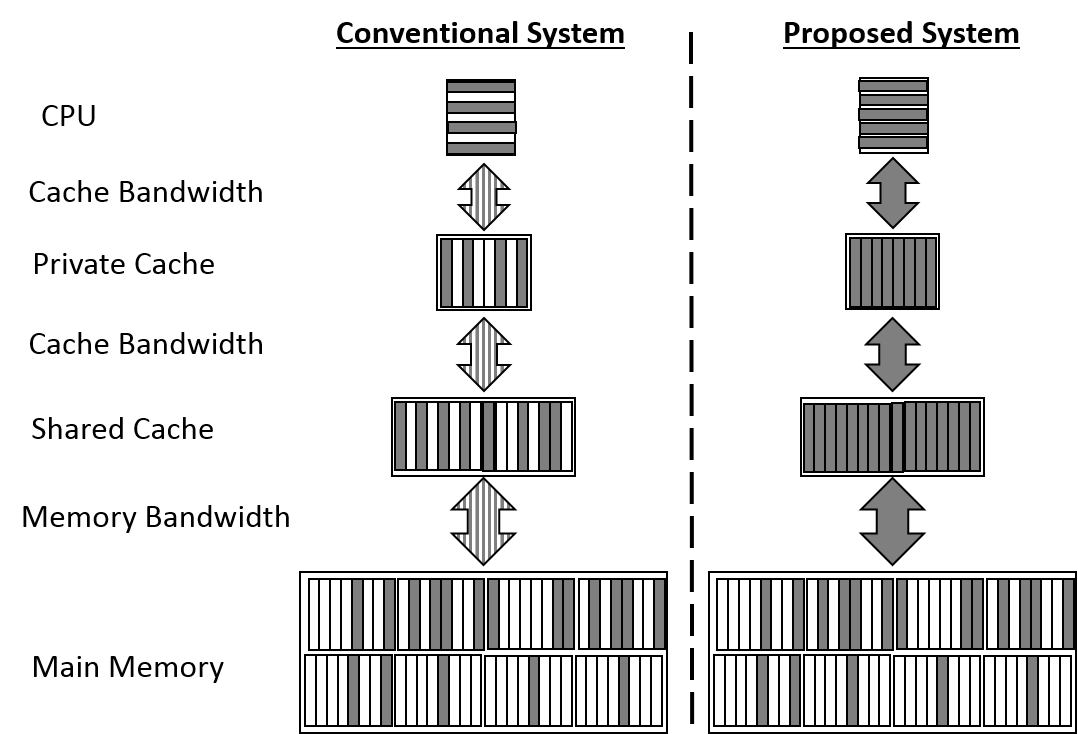
\includegraphics[width=3.4in]{Figures/system-comparison.png}
\caption{Processor and memory system utilization of sparse (white) and non-sparse (shaded) data.}
\label{fig:system-compare}
\end{figure}

Our proposed optimizations can improve DNN training peformance and scalability in three ways.  First, by eliminating computations on useless data while processing a training example, more iterations over the data set can be completed within a time budget (e.g., a week), which can improve model quality.  Second,  memory system  bandwidth is a key bottleneck for {\it data-parallelism} within a machine (i.e., processing multiple examples at once using multiple CPU cores). By reducing the bandwidth utilization for each example, data-parallelism can scale training throughput more effectively.  Finally, a standard approach for fitting big DNN models into the last level cache is partitioning the model across multiple machines to exploit the aggregate cache capacity (a.k.a., {\it model-parallelism}). By reducing the cache consumption of a model partition, our techniques can increase the per-machine partition size and reduce the number of machines required to achieve a target training throughput, reducing model parallelism costs. 

Prior software~\cite{Eisenstat82, IntelSparseMatrix} and hardware~\cite{Carter99, Srinidhi12, Fowers13} approaches for spare data computations are less effective for DNN training for two reasons.  First, those techniques assume that sparsity exists only in matrices but not in vectors, whereas in DNN training both matrices and vectors can be sparse.  Second, those techniques assume that the sparse data structures are static, so that the cost of constructing a sparse representation is amortized over many uses.  However, the matrices and vectors in DNN training change for each training example, thus representation cost is incurred repeatedly, hurting performance. 

Our approach consists of processor and memory system techniques for reducing sparse data computation overheads.  Our processor extensions are based on ``zero-optimizable'' instructions, which are arithmetic instructions (e.g., multiplication) with predetermined results and side effects when an input operand is zero. Our optimizations reduce execution cycles and processor resource pressure by skipping instructions (including entire loops) that become redundant because of a zero input to a zero-optimizable instruction.  Our memory system extensions efficiently track zero data at cache line granularity to avoid the storage and bandwidth costs of zero cache lines.  Our approach is transparent to software and therefore benefits existing binaries. 

We evaluate our proposed hardware extensions in a simulation environment using real-world DNN training workloads for image recognition. The results show significant improvements in training time in single threaded, multi-threaded, and model-parallelism scenarios.

This paper makes the following contributions.
\begin{itemize}

\item We propose new hardware techniques for improving the performance and scalability of DNN training by reducing computational requirements of sparse data computations, without requiring software changes.  We present a detailed design of our proposed hardware extensions, which add negligible logic on the critical path of processor execution and memory accesses. 
\item We study the impact of sparse data on computation in a real-world DNN training for an image recognition task. We show that eliminating such unnecessary computations can greatly improve performance and scalability of such a real-world workload.
\item We quantitatively evaluate how our optimizations improve DNN training peformance and scalability using standard image recognition workloads. 

\end{itemize}

The rest of the paper is organized as follows.  Section~\ref{sec:background} provides background on DNN and DNN training.  Section~\ref{sec:sparse_dnn_training} studies spare data computations in DNN training.  Our processor optimizations are described in Section~\ref{sec:processor_opt}, while our cache optimizations are described in Section~\ref{sec:cache_opt}.  We present our evalutation results in Section~\ref{sec:eval}, review related work in Section~\ref{sec:related},  and conclude in Section~\ref{sec:conclude}.



\section{Background}
\label{sec:background}

\subsection{Deep Neural Networks}
\label{subsec:dnn}
DNNs consist of large numbers of neurons with multiple inputs and a single output called an activation. Neurons are connected hierarchically, layer by layer, with the activations of neurons in layer $l-1$ serving as inputs to neurons in layer $l$.  This deep hierarchical structure enables DNNs to learn complex AI tasks, such as image recognition, speech recognition and text processing~\cite{Bengio09}. DNNs comprise {\it convolutional} layers (possibly interleaved with {\it pooling} layers) at the bottom of the hierarchy followed by {\it fully connected} layers.  Convolutional layers, which are inspired by the visual cortex~\cite{Hubel59}, extract features from input samples, and consist of neurons that are only connected to spatially local neurons in the lower layer~\cite{LeCun98b}.  Pooling layers summarize the features learned by convolutional layers (e.g., identify the maximum intensity in a cluster of image pixels, reduce spectral variance in speech samples).  Fully connected layers classify the learned features into a number of categories (e.g., handwritten digits) and consist of neurons that are connected to all neurons in the lower layer.

\subsection{DNN Training}
A common approach for training DNNs is using  learning algorithms, such as stochastic gradient descent (SGD)~\cite{Bottou10}, and labeled training data to tune the neural network parameters for a specific task. The parameters are the {\em bias} of each neuron and the {\em weight} of each neural connection. Each training input is processed in three steps: {\em feed-forward evaluation}, {\em back-propagation}, and {\em weight updates}.

{\bf Feed-forward evaluation:}
Define $a_{i}$ as the activation of neuron $i$ in layer $l$. It is computed as a function of its $J$ inputs from neurons in the preceding layer $l-1$:
\begin{equation}
{\it a_{i}} = f\left(\left(\sum\limits_{j=1}^{J}{\it w_{ij}} \times {\it a_{j}}\right) + {\it b_{i}}\right) \ ,
\label{eqn:fwd_activation}
\end{equation}
where $w_{ij}$ is the weight associated with the connection between neurons $i$ at layer $l$ and neuron $j$ at layer $l-1$, and $b_{i}$ is a bias term associated with neuron $i$. The activation function, $f$, associated with all neurons in the network is a pre-defined non-linear function, typically sigmoid or hyperbolic tangent.

{\bf Back-propagation:}
Error terms $\delta$ are computed for each neuron $i$ in the output layer $L$:
\begin{equation}
\delta_{i} = \left(true_{i} - a_{i}\right) \times f'(a_{i})\ ,
\label{eqn:output_error_term}
\end{equation}
where $true(x)$ is the true value of the output and $f'(x)$ is the derivative of $f(x)$.
These error terms are back-propagated to each neuron $i$ in the layer $l$ from its $S$ connected neurons in layer $l+1$:
\begin{equation}
\delta_{i} = \left(\sum\limits_{s=1}^{S}\delta_{s} \times w_{si}\right) \times f'(a_{i}) \ .
\label{eqn:other_error_term}
\end{equation}

{\bf Weight updates:}
These error terms are used to compute the weight deltas, $\Delta w_{ij}$, for updating the weights:
\begin{equation}
\Delta w_{ij} = \alpha \times \delta_{i} \times a_{j} ~~for~ j = 1...J \ ,
\label{eqn:weight_delta}
\end{equation}
where $\alpha$ is the learning rate and $J$ is the number of neurons of the layer.  

This process is repeated for each input until the entire training data has been processed, which constitutes a training {\it epoch}. Typically, training continues for multiple epochs, reprocessing the training data set each time, until the error converges to a desired (low) value.

\section{Sparsity in DNN Training}
 \label{sec:sparse_dnn_training}
 
 We motivate our work and project the benefits of our optimizations for DNN training.  First, we provide intutition into why sparsity exists in DNN training.  Next, using a real-world image recogntion workload, we empirically demonstrate the amount of sparsity that exists in practice.  Finally, we discuss how available sparsity can be exploited using our techniques to improve training efficiency. 
 
\subsection{Sources of Sparsity}
\label{subsec:sparsity_source}

Machine learning experts have long observed that DNN training using back-propagation and gradient descent involves a considerable amount of computation on sparse data structures~\cite{Ng04, Nair10, Krizhevsky12, Bengio13, Srivastava14a} (i.e., data structures that contain a significant fraction of zeroes).  Specifically, performance-critical data of training, such as error gradients and weight deltas, can exhibit noticeable levels of sparsity during training.   Some of the sparsity arise naturally from the training algorithm  and the underlying matrix multiplication kernels.  For example, correct predictions of a neuron's output activation during feed-forward evaluation results in zero-valued neuron error gradients, during back-propagation, which can introduce sparsity in the rest of the network.  Beyond this, standard techniques for boosting training quality often introduce additional sparsity in the network.  These include techniques such as Rectified Linear Units (ReLUs)~\cite{Nair10, Krizhevsky12} for faster convergence, and  L$_1$~\cite{Ng04, Bengio13} and Dropout~\cite{Srivastava14a} regularization methods for reducing overfitting. 

\subsection{Sparsity in Real-word Image Recognition}
\label{subsec:sparsity_profile}

To provide insight into the amount of sparsity that exists in real-world DNN training workloads, we profile the training of a DNN model on the standard {\it CIFAR-10} image recognition task~\cite{KrizhevskyThesis} (described in ~\ref{subsec:eval_method}).  In our study, we reason about sparsity from two perspectives: (i) computation sparsity and (ii)  data sparsity.  Computation sparsity measures the percentage of mutiply-add operations that are performed on zero values in the performance-critical phases of training (e.g., feed-forward evaluation), while data sparsity measures the percentage of zeroes in the input data (e.g., activations) of these phases.  Both perspectives are useful because they capture different impacts of sparsity on system performance, and motivate different optimization opportunities.  Computation sparsity captures the impact on processing cycles, data sparsity captures the impact on memory capacity, and both metrics capture the impact on memory bandwidth.  We measure both sparsity metrics over $10$ training epochs using the standard training data set of $60000$ images. 

\begin{figure*}
 \centering
 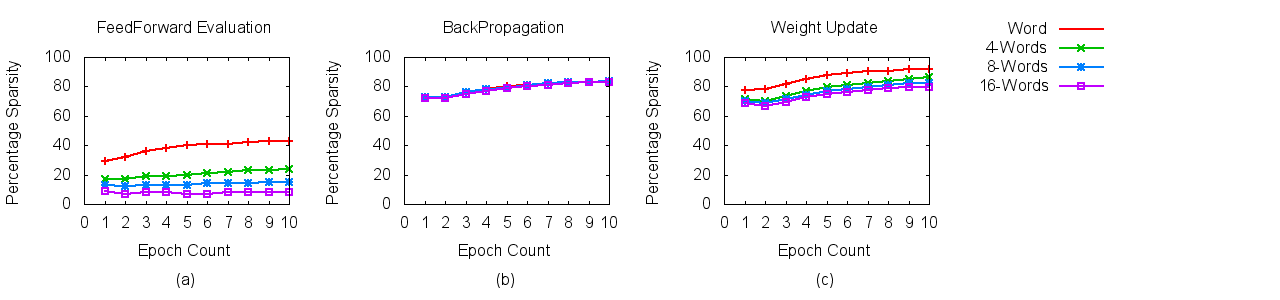
\includegraphics[width=1.9\columnwidth]{Figures/multi_computesparsity.png}
\caption{Computation sparsity in CIFAR-10 image recognition training.}
 \label{fig:cifar-10_compute_sparsity}
 \end{figure*}
 
\subsubsection{Computation Sparsity}
\label{subsec:computation_sparsity}
 Figure~\ref{fig:cifar-10_compute_sparsity} reports computation sparsity in the key phases of DNN training for the first $10$ epochs of training a CIFAR-10 image recognition model.  Since computation sparsity represents opportunities to safely reduce processing cycles, Figure~\ref{fig:cifar-10_compute_sparsity} reports sparsity for different computation granularities to show the potential benefits for non-vectorized (i.e., {\it Word}) and vectorized (e.g., {\it 4-Words}) implementations of the computation kernels.  For example, for feed-forward evaluation, {\it Word} sparsity is the percentage of CPU multiply-adds that can be skipped because one of the input activation or weight values is zero, while {\it N-Words} sparsity is the percentage of N-wide vector (SIMD) multiply-adds that can be skipped because either the $N$ activation values or $N$ weight values are zero. 
 
We make the following four observations regarding computation sparsity in DNN training from Figure~\ref{fig:cifar-10_compute_sparsity}.  First, considerable sparsity exists in all the training phases: {\it Word} sparsity is $29\%$---$43\%$ for feed-forward evalution, $73\%$---$84\%$ for backpropagation, and $77\%$--$92\%$ for weight updates.   Second, the training phases have different amounts of computation sparsity, with feed-forward evaluation having the least amount of computation sparsity. Third, computation sparsity generally \emph{increases} with epoch count.  Fourth, vectorization affects computation sparsity of the training phases in different ways: vectorization has no impact on sparsity for backpropagation, but reduces sparsity modestly for weight updates and significantly for feed-forward evaluation (e.g., {\it 4-Words} sparsity is half of {\it Word} sparsity).  In summary, the results shows there is potential to greatly reduce the processing and memory bandwidth requirements of DNN training by exploiting computation sparsity, but vectorization limits the benefits for feed-forward evaluation. 

%Fourth, the impact of vectorization on computation sparsity varies across the training phases: no impact for backpropagation, modest sparsity reduction for weight updates, and significant sparsity reduction for feed-forward evalution (e.g., {\it 4-Words} sparsity is half of {\it Word}).  In summary, the results shows there is potential to greatly reduce the processing and memory bandwidth requirements of DNN training by exploiting computation sparsity, but vectorization limits the benefits for feed-forward evaluation. 
  
 \begin{figure*}
 \centering
 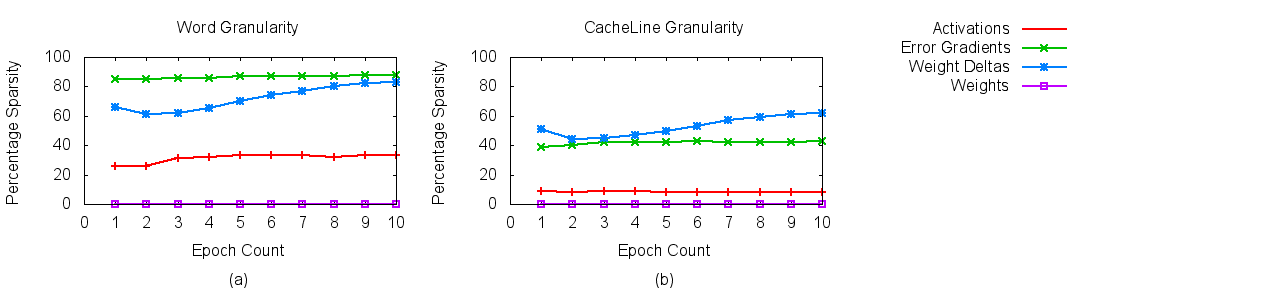
\includegraphics[width=1.9\columnwidth]{Figures/multi_datasparsity.png}
\caption{Data sparsity in CIFAR-10 image recognition training.}
 \label{fig:cifar-10_data_sparsity}
 \end{figure*}

\subsubsection{Data Sparsity} 
\label{subsec:data_sparsity}
Figure~\ref{fig:cifar-10_data_sparsity} reports the sparsity of the different performance-critical data in DNN training: (i) activations, (ii) error gradients, (iii) weight deltas, and (iv) weights (defined in Section~\ref{subsec:dnn_training}).  The results are presented for word and cacheline granularities.  Data sparsity at word granularity is the percentage of individual data values (e.g., activations) which are zeroes, while cacheline granularity is the percentage of data cache lines containing only zeroes.  Since training data values are represented with 4-byte floats, the $64$-byte cacheline granularity represents clusterings of $16$ sparse data values.  Viewing data sparsity at both word and cacheline granularities helps one understand the trade-offs of different optimization strategies since significantly more expensive hardware is required to track sparsity at word granularity compared to cacheline granularity.  

We make the following three observations regarding data sparsity in DNN training from Figure~\ref{fig:cifar-10_data_sparsity}.  First, sparsity level varies across the different data items: at word granularity, weights have $0\%$ sparsity (i.e., dense), while activations ($26\%$---$33\%$), error gradients ($83\%$---$85\%$), and weight deltas ($66\%$---$83\%$) are considerably sparse.   Second, for the sparse data items, sparsity tends to increase with more training epochs.  Third, sparsity levels are reduced at cacheline granularity to about half of word granularity, which suggests poor clustering of sparse data values in the data layout of the workload.  However, considerable levels of sparsity \emph{stil}l remain at the cacheline granularity.  In summary, the results show that cache capacity and bandwidth requirements of DNN training can be greatly reduced by exploiting data  sparsity, even at the relatively large cacheline granularity.

\subsection{Optimization Opportunities}
\label{subsec:sparse_code_oppor}
We motivate our hardware optimizations for sparse data computations in DNN training by studying a performance-critical kernel for computing weight deltas in back-propagation.  Figure~\ref{fig:deltas_source_code} illustrates a simplified version of this kernel.\footnote{Our approach also applies to vectorized (e.g., SIMD) kernels, but we use the simple forms in our discussion for convenience.}   The weight deltas of a layer in the DNN are computed by the inner product of the neuron activations and error gradients.  Given the amounts of computation and data sparsity in training, a promising optimization for this kernel is to skip the multiply-add operations if either \emph{activations[i]} or \emph{errors[j]} is zero.  Moreover,  if \emph{errors[j]} is zero, the inner loop can be skipped entirely since \emph{errors[j]} is loop-invariant. These optimization ideas also apply to the other performance-critical kernels of training, e.g., feed-forward evalution. 

\begin{figure}[h]
 \centering
 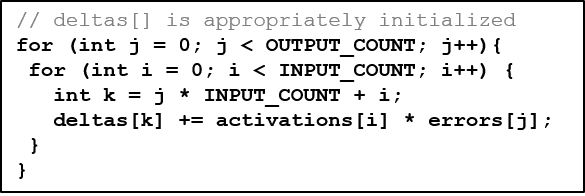
\includegraphics[width=.9\columnwidth]{Figures/deltas_source_code.png}
\caption{Code snippet for computing weight deltas.}
 \label{fig:deltas_source_code}
 \end{figure}

Although these optimizations could be implemented in software by checking the data values for zero and guarding computations based on those checks, such a software approach has a couple of practical limitations.   First, it requires software changes which might not be possible for existing binaries.   Second, the required software checks incur both computation and memory overheads, which could be significant and outweigh the optimization benefits.  For example, checking \emph{activations[i]} and checking \emph{errors[j]} for zeroes have different performance impact.  Checking \emph{errors[j]} for zeroes is likely to be beneficial because it can be done \emph{outside} the inner loop, and helps to skip large amounts of computation. In contrast, checking \emph{activations[i]} for zeroes will likely hurt performance because it occurs \emph{inside} the inner loop, and can save only a small amount of computation. Our hardware optimizations  avoid such limitations and overheads.  We compare the performance benefits of software and hardware approaches in our evaluation (Section~\ref{sec:eval}). 


\subsubsection{Our Goal and Overview of our mechanisms}

%\section{Overview}
\label{sec:overview}

We now present an overview of our hardware approach for improving system performance by reducing or eliminating the overheads of sparse data computations in DNN training. Our technique comprises of extensions to the processor and memory systems that enable more efficient handling of zero data values and associated computations.  

\subsection{Processor Optimizations}
Our processor optimizations are based on the observation that the results of addition and multiplication operations---the core part of DNN training kernels---can be determined without performing the operation if one of the input operands is a zero.  We refer to instructions that perform these arithmetic operations with at least one zero-value input operand as ``zero-optimizable'' instructions.  In modern out-of-order processor pipelines, a zero-optimizable in the instruction queue presents a number of optimization opportunities because its result and side effects can sometimes be determined once the zero input operand becomes available. In particular, a zero-optimizable instruction could render some data dependencies and pipeline stages redundant, making it possible to non-speculatively issue or commit instructions earlier than normal or even squash instructions. We discuss these optimization opportunites in more details below using the DNN training code snippets in Figure~\ref{fig:gradient_code} to motivate the ideas.  Figure~\ref{fig:gradient_code}(a)  shows source code for error gradient computation, while Figure~\ref{fig:gradient_code} (b) shows the inner loop using sample machine instructions.  In the discussion below, we  assume that R$0$, which corresponds to errors[i] in the source code,  is zero in the loop. 

\subsubsection{Early Instruction Issue/Commit.}  First, a zero-optimizable instruction can be issued once the zero operand is available if the zero makes other operands redundant.  For example, I$4$ is a zero-optimizable instruction which can be issued early becaue it is a multiplication and the zero value of R$0$ makes R$2$ redundant.  Second, a zero-optimizable instruction could be committed early if the zero input determines its results and side effects. This is the case for I$4$. Early issue and commit of zero-optimizable instructions can reduce pressure on processor resources and wait times of data dependent instructions, such as I$5$, since the dependencies are satisfied sooner. 

\subsubsection{Instruction Squashing.} A zero-optimizable instruction can be squashed in the instruction queue if a zero input operand makes it an identity function and thus redundant. For this reason, I$5$ can be quashed since it is an addition and R$2$ is zero. Since a squashed instruction can make redundant other instructions that it depends on (producers) and that depend on it (consumers),  quashed zero-optimized instruction can make dependent instructions redundant as well.  For example, I$6$ is redundant and can be squashed since it is effectively a silent store. 
 



\begin{comment}
\begin{figure}[!t]
\centering
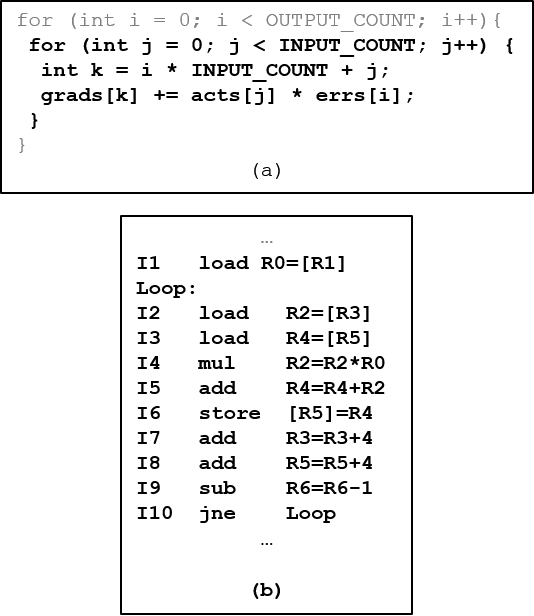
\includegraphics[width=2.4in]{Figures/gradient_code.png}
\caption{(a) Source code for computing error gradients and (b) corresponding machine instructions of inner loop.}
\label{fig:gradient_code}
\end{figure}
\end{comment}

\begin{figure*}
\centering
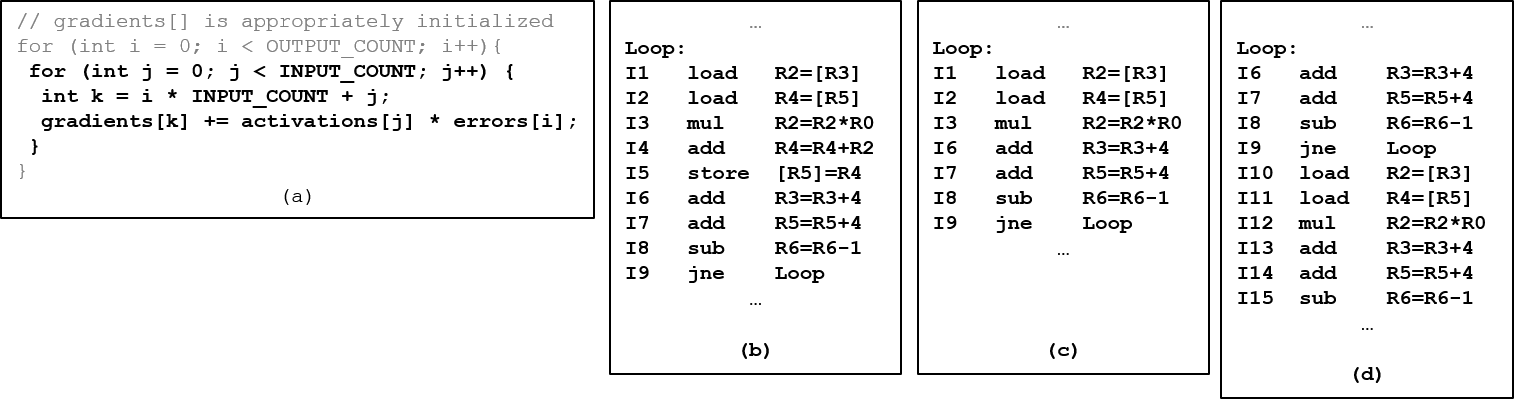
\includegraphics[width=1.9\columnwidth]{Figures/gradient_code_opt.png}
\caption{(a) Source code for computing error gradients, (b) machine code of inner loop, (c) optimized code after basic instruction quashing, and (d) optimized code after advanced instruction quashing.}
\label{fig:gradient_code}
\end{figure*}


\subsection{Memory System Optimizations}


 
 

%\section{Hardware Design}
\label{sec:design}

We now describe the hardware extensions for implementing our proposed processor and memory system optimizations.

\subsection{Processor Extensions}



\subsection{Memory System Extensions}

%\section{Processor Optimizations}
\label{sec:processor_opt}

Our processor optimizations are based on arithmetic operations, such as addition and multiplication, which are performance critical in training computations, and have predetermined results when one of the input operands is a zero. We refer to machine instructions that perform such arithmetic operations as ``zero-optimizable'' instructions. Exploiting zero-optimizable instructions to improve training peformance is promising because, as shown in our profiling studies (Figure~\ref{fig:cifar-10_word_sparsity}), a significant portion of the inputs to training computations are zeroes. 

\begin{figure}
\centering

\includegraphics[height=1.4in, width=.9\columnwidth]{Figures/gradient_machine_code.png}
\caption{(a) original and (b) optimized machine code of gradient computation inner loop.}
\label{fig:gradient_code_opt}
\end{figure}

\subsection{Opportunities}

We discuss the dynamic optimization opportunities that motivate our processor techniques using the machine code sequences in Figure~\ref{fig:gradient_code_opt}, which correspond to the inner loop of the gradient computation code in Figure~\ref{fig:gradient_source_code}.    Figure~\ref{fig:gradient_code_opt}(a) represents machine code that is generated by a static compiler\footnote{Our optimizations also apply to loop optimizations (e.g., unrolling).}, and consists of five zero-optimizable instructions: I$3$, I$4$, I$6$, I$7$, and I$8$.  Figure~\ref{fig:gradient_code_opt}(b) shows the code sequence resulting from dynamic optimization of the loop using our techniques when the loop invariant input of I$3$, R$0$ (i.e., \emph{outputErrors[j]} in Figure~\ref{fig:gradient_source_code}), is zero.  We now describe how our dynamic techniques improve performance using zero-optimizable instructions with zero input values. 

\subsubsection{Zero-Optimizable Instructions.} A zero-optimizable instruction presents a number of opportunities to increase ILP and reduce resource pressure of training workloads on modern out-of-order processors.  These opportunities arise because of the predetermined results of zero-optimizable instructions when computing on zero input operands.  Since we focus on zero-optimizable instructions performing additions or multiplications, we consider how these instructions could be affected by a zero input when there are two input and one output operands.  

 A zero input operand converts an addition instruction into a copy operation of the other input operand into the destination location. Also, if the other input operand is also the destination operand then the copy operation is redundant.  For multiplications, a zero input operand results in a zero value of the destination operand regardless of the value of the other input operand.  Thus, zero input operands can make some data dependencies and pipeline stages redundant for zero-optimizable and dependent instructions.  Consequently, zero-optimizable and dependent instructions can be issued or commited earlier than normal or eliminated completely, as discussed below. 

\subsubsection{Early Instruction Issue/Commit.}  First, a zero-optimizable instruction can be issued once the zero operand is available if it makes other operands redundant.  For example, I$3$ can be issued early becaue it is a multiplication and the zero value of R$0$ makes R$2$ redundant.  Second, a zero-optimizable instruction could be committed early if the zero input determines its results and side effects. This is also the case for I$3$. Early issue and commit of zero-optimizable instructions can reduce pressure on processor resources and wait times of data dependent instructions, such as I$4$, since the dependencies are satisfied sooner. 

\subsubsection{Instruction Elimination.} A zero-optimizable instruction can be squashed in the instruction queue if a zero input operand makes it an identity function and thus redundant. For this reason, I$4$ can be squashed since it is an addition and R$2$ is zero. Squashing an instruction can make the  instructions that it depends on (producers) and those that depend on it (consumers) redundant, leading to more instruction squashing.  For example, I$5$ becomes redundant (a silent store) and can be squashed, if I$5$ is squashed. Figure~\ref{fig:gradient_code_opt}(c) shows the impact of squashing I$4$ and I$5$.  We further observe that  I$1$, I$2$, and I$3$ are now redundant in all but the last loop iteration, since their results (R$2$ and R$4$) are not used.  We can squash these three instructions in all but the last iteration as shown in Figure~\ref{fig:gradient_code_opt}(d). Compared to the orignal machine code sequence, the optimized code sequence will run much faster because of the squashed instructions, especially loads which often have high latency.  Thus, by exploiting zero-optimizable instructions we can improve the performance of the inner loop of the gradient computation code. 

\subsection{Mechanisms}

We propose extensions to a modern OOO pipeline for dynamic optimization of zero-optimizable instructions and the loops containing them.  Our optimizer system comprises of lightweight extensions in the front-end and heavyweight extensions in the back-end of the pipeline.  The split into lightweight and heavyweight components helps to avoid critical path delays in the front-end, while extracting maximum performance improvements.  The front-end extensions enable early instruction issue/commit, while the back-end extensions enable instruction squashing in loops.  Figure~\ref{fig:opt_pipeline} presents an overview of augmenting a standard OOO six-stage pipeline with our optimization system.

\begin{figure}
\centering
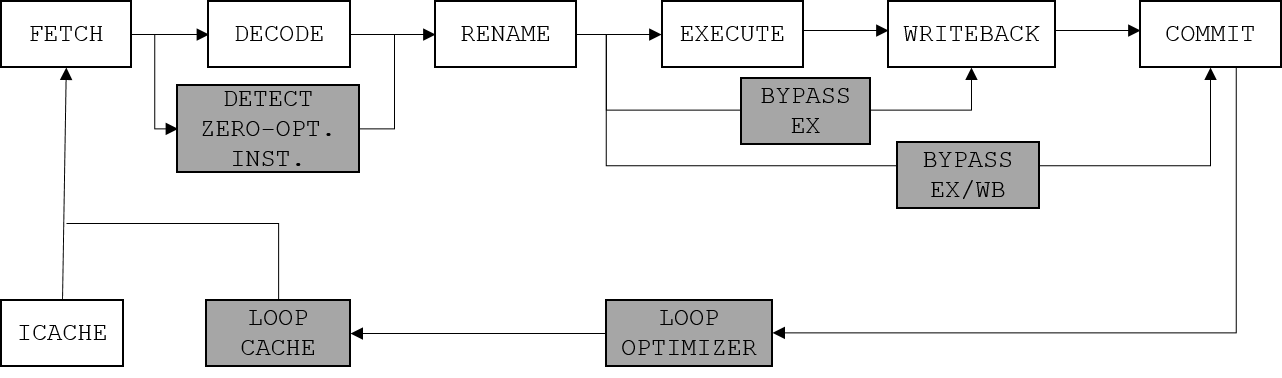
\includegraphics[height=1in]{Figures/pipeline.png}
\caption{Overview of processor extensions.}
\label{fig:opt_pipeline}
\end{figure}

\subsubsection{Front-End Extensions.}
The objectives of the front-end extensions are the following: (i) detect zero-optimizable instructions in the instruction stream and (ii) bypass pipeline stages.  These steps can be done in parallel with existing pipeline stages, as discussed below.  

\paragraph{Detect Zero-optimizable Instructions.}
This is done in the decode stage by matching the instruction opcode against a predefined set of opcodes. Since the opcode set is small, i.e., addition and multiplication opcodes, the matching can be done in parallel to avoid extra delays.  The zero-optimizable instructions detected here are marked for easy identification in later pipeline stages. 

\paragraph{Bypass Pipeline Stages.}
We exploit zero operand values to bypass the execute and writeback stages whenever possible.  This is done while a zero-optimizable instruction is in the instruction queue waiting for data dependencies.  We extend the mechanism for detecting operand availability to also check whether or not the value is zero.  For a multiplication instruction or a redundant addition instruction (i.e., destination operand is same as other source operand), we break outstanding data dependencies of the instruction making the instruction ready to issue.  We extend the issue logic to allowing issuing instructions directly to stages later than the execute stage.  This allows us to issue multiplication instructions to the writeback stage to zero the destination operand (and broadcast availability), and issue redundant additions to the commit stage.   

%Our approach performs the following operations in the pipeline front-end: (i) identify zero-optimizable instructions, (ii) detect when zero-optimizable input operand is a zero, (iii) modify producer and consumer data dependencies, and (iv) squash instructions.  These steps can be done in parallel with existing pipeline front-end stages, as we discuss below. 

%\subsubsection{Identify Zero-Optimizable Instructions.} We can detect zero-optimizable instructions during instruction decoding by matching the opcode against a predefined set of opcodes. Since only a small set of arithmetic instructions qualify as zero-optimizable, the storage requirements of the opcode set is modest, and opcode matching can be done in parallel to avoid extra delays. Zero-optimizable instructions that are identified in the decode stage are marked for easy identification in later pipeline stages. 

%\subsubsection{Detect Zero Operands.} We can detect zero input operands while a zero-optimizable instruction is waiting in the instruction queue for data dependencies.  Current mechanisms for signaling operand availability can be extended to also indicate whether or not the value is zero. 
 
 %\subsubsection{Modify Data Dependencies.}  We can extend current mechanisms for tracking data dependencies among instructions to clear dependencies of zero-optimizable instructions that become redundant due to a zero input operand becoming available. Futhermore, dependencies from instructions that consume the results of a zero-optimizable instruction should be cleared when a zero input makes the instruction an identity function, and thus redundant.  
 
 \subsubsection{Back-End Extensions.}
 Our backend extensions consists of two components: (i) a mechanism for detecting and optimizing loops based on zero-optimizable instructions, and (ii) an optimized loop code cache.  The goal is to eliminate instructions that are made redundant by zero inputs to zero-optimizable instructions in the loop.  Thus, the optimized loop code is smaller than the original loop 
 
 \paragraph{Loop Optimizer.} This mechanism scans the stream of committed instructions to detect loops that can be optimized based on zero-optimizable 
 
 \paragraph{Optimized Loop Code Cache.} This mechanism caches the optimized code sequences generated by the loop optimizer and ensures the cached sequences are executed in place of the original code sequences.   
 
 

\section{Processor Optimizations}
\label{sec:processor_opt}

\subsection{Back-End Extensions}
Our backend extensions perform three critical functions in the optimization of DNN training code: (i) generate optimized versions of loops in the training code based on computation sparsity, (ii)  for each loop that is optimized, maintain a lookup table of the optimized versions which the frontend uses to redirect execution to optimized codes,  and (iii) maintain a code cache for storing optimized loop codes. 

\subsubsection{Generating Optimized Loop Codes}
The goal of the optimizer is to generate more efficient versions of the loops in the training code that will boost training performance when executed in place of the original loop codes.  The efficient loop versions are obtained by by applying aggressive loop optimizations that are predicated on assumptions of sparsity in loop data and computation.  Thus, the optimized loop codes can only be executed when the underlying conditions hold true. 


The goal of the optimizer is to generate efficient versions of the loops in the training code, and coordinating with the frontend to ensure that an optimized version of a loop is executed instead of the original only in the right conditions.   Our loop optimizations are predicated on the condition that an input data of the loop is zero,  and so the optimized loop version can only be executed when that condition holds.  

\begin{figure}[h]
\centering
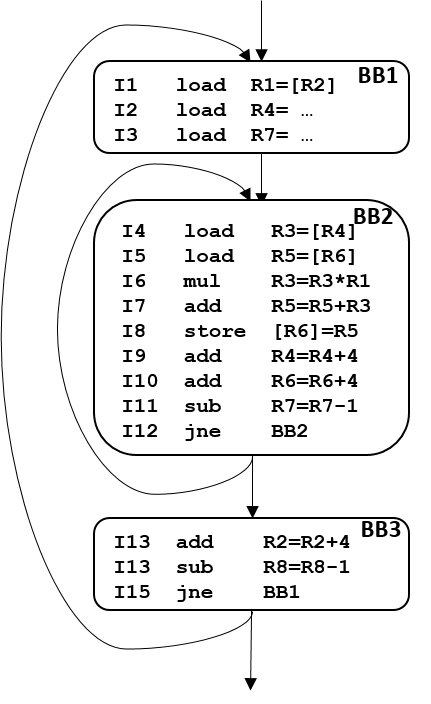
\includegraphics[height=1.8in]{Figures/weight-delta-code.png}
\caption{Code forcomputing  weight deltas (Figure~\ref{fig:deltas_source_code}).}
\label{fig:deltas_machine_code}
\end{figure}


\subsubsection{Executing Optimized Loop Codes}


\begin{figure}[h]
\centering
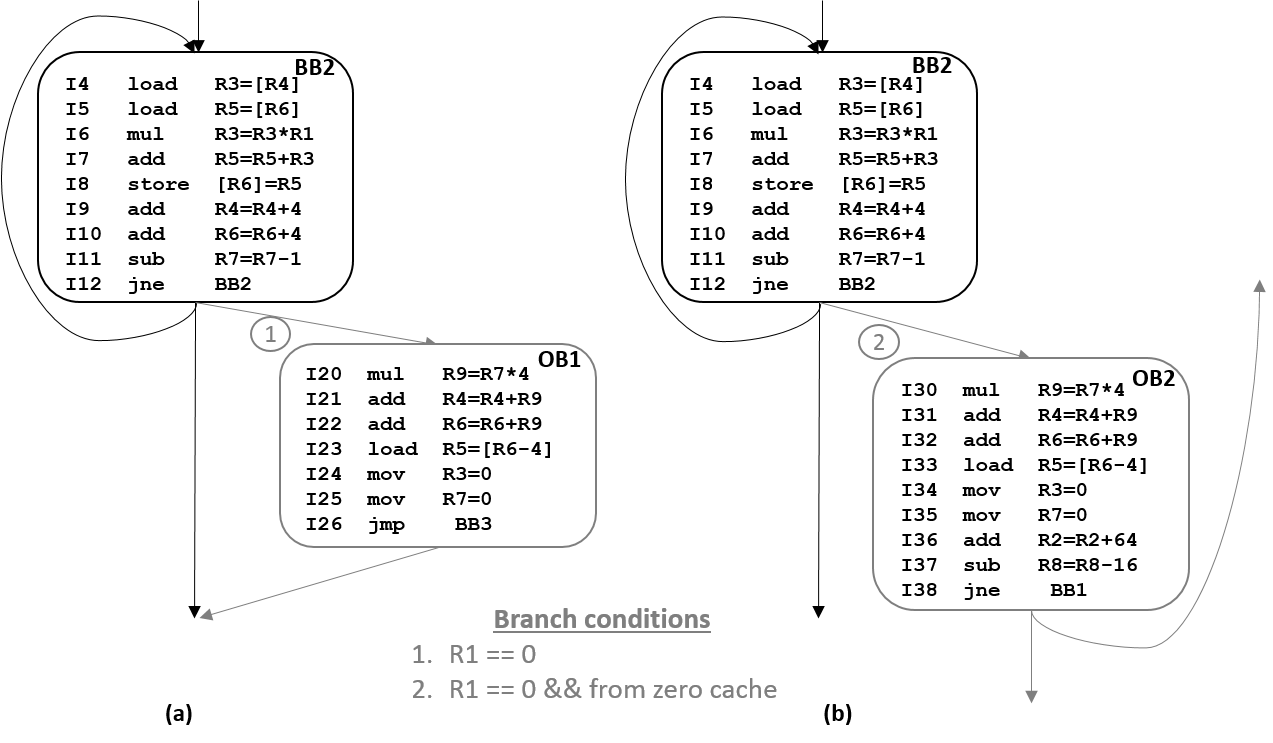
\includegraphics[height=1.8in, width=.95\columnwidth]{Figures/loop-invariant-zopt.png}
\caption{Optimizing for loop invariant zero data (R1): (a) for data from data cache, redirect execution to skip inner loop, and (b) for data from zero cache (i.e., cluster of $16$ zero data values) redirect execution to skip 16 executions of inner loop.}
\label{fig:deltas_loop_inv_opt}
\end{figure}



\begin{figure}[h]
\centering
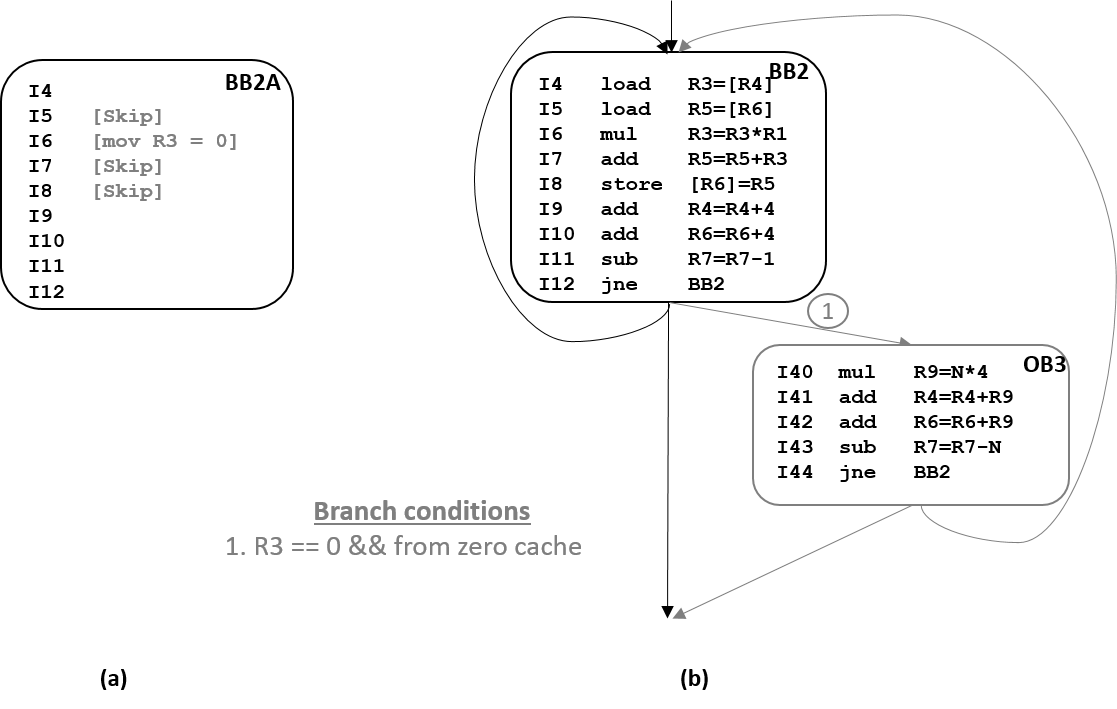
\includegraphics[height=1.8in, width=.95\columnwidth]{Figures/loop-variant-zopt.png}
\caption{Optimizing for loop variant zero data (R3):  (a) annotate code block actions to be taken by frontend, and (b) redirect execution for data from zero cache.}
\label{fig:deltas_loop_var_opt}
\end{figure}

\subsubsection{Storing Optimized Loop Codes}


\subsection{Front-End Extensions}

\section{Cache Optimizations}
\label{sec:cache_opt}

Our cache optimizations for DNN training are based on the sparse nature of the performance critical data (in Figure~\ref{fig:cifar-10_data_sparsity}).  Our approach improves cache performance through a compact representation of cache lines containing only zeroes (a.k.a. \emph{zero cache lines}) in the caches, which helps to avoid  the normal bandwidth and storage costs of zero cache lines. These optimizations enable efficient scaling of model size and training threads.  

Managing zero data at cache line granularity enables implementation of our optimizations through simple and efficient extensions of existing memory systems.  Our design comprises of new mechanisms for: (i) compact representation of zero cache lines, (ii) a decoupled cache hierarchy for zero cache lines, and (iii) tracking zero cache lines in the memory system.  We describe these mechanims in the rest of this section.

\begin{figure}[!t]
\centering
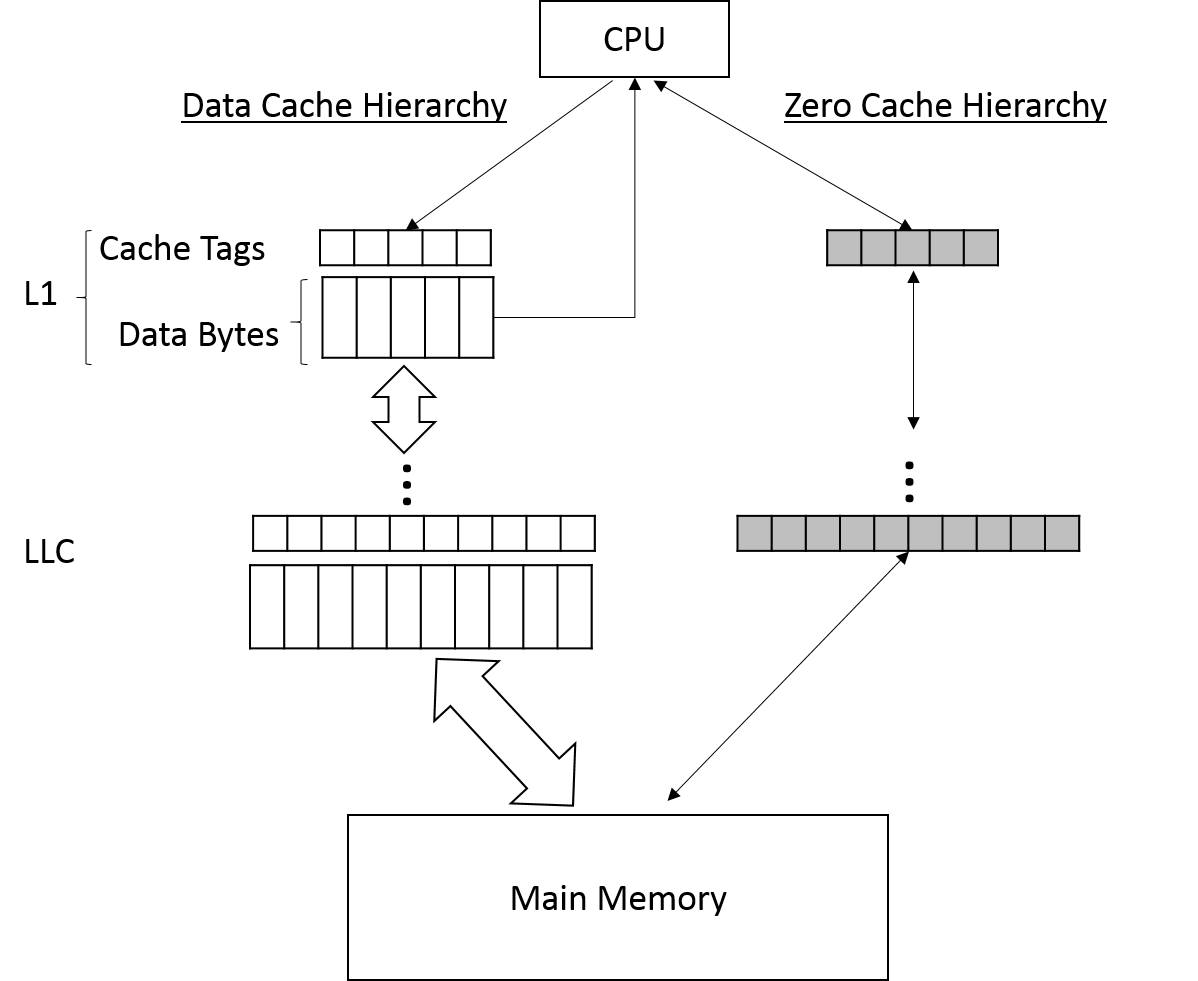
\includegraphics[width=2.4in]{Figures/zero_cache_hierarchy.png}
\caption{A Memory System with Zero Cache Hierarchy.}
\label{fig:zero_cache_hierarchy}
\end{figure}

\subsection{Zero Cache Line Representation}

Our compact representation exploits the fact that the data bytes of a zero cache line are not required to represent the line in cache.  The cache tag is sufficient for this purpose. Also, it is not neccesary to transfer the data bytes of a zero cache line across the caches since they can be synthesized in the processor (read) or main memory (on a writeback) as appropriate.  However, in the event of a cache hit, we must quickly determine whether it is a zero cache line that is referenced so that the appropriate data transfer, if need (i.e., non-zero),  is done promptly. We consider two alternatives for handling this: (i) an extra bit in the cache tag to identify a zero cache line or (ii) a decoupled hierarchy of cache tags for zero cache lines.  Although the first option avoids the extra cost of zero cache line tags, the data store space of zero cache lines goes unused.  To avoid this waste, we adopt the second option in our current work. 

\begin{figure}[!t]
\centering
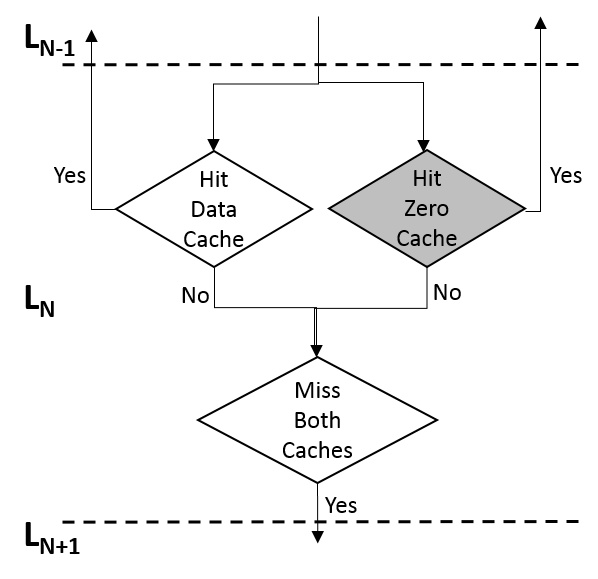
\includegraphics[ height=2in]{Figures/cache_access_flowchart.png}
\caption{Handling read requests.}
\label{fig:cache_access_flowchart}
\end{figure}

\subsection{Hierarchy of Zero Cache Lines}

Figure~\ref{fig:zero_cache_hierarchy} illustrates a memory system that is augmented with a cache hierarchy for zero cache lines, which we call the \emph{zero cache} hierarchy. The zero cache hierarchy is a multi-level structure with caches (a.k.a., \emph{zero caches}) containing tags but no data bytes.  Since zero cache lines are not maintained in the conventional data caches, both cache hierarchies are mutually exclusive. The zero cache hierarchy and the data cache hierarchy have the same number of levels, and can additionally share other properties, such as number of entries, ways, associativity, replacement policies, etc.  The coherence of zero caches is maintained across cores using the same protocol as the data caches. 

Data access requests from the processor are satisfied by accessing the two cache hierarchies in parallel to avoid introducing extra latency. Figure~\ref{fig:cache_access_flowchart} shows the processing of a read request by the $N$th level caches.  The request is processed in parallel by the data  and zero caches, and forwarded to the next level if it is a miss in both.  If the request is a hit in either cache, then the appropriate response is sent to the processor or lower levels of the cache hierarchy.   The data cache responds, as normal, with the requested data bytes (or cache line), while the zero cache responds by signaling a zero cache line hit. 

\begin{figure}[!t]
\centering
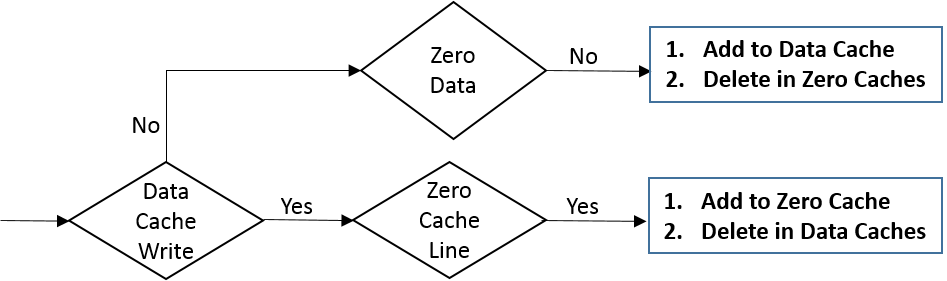
\includegraphics[width=0.9\columnwidth]{Figures/processor_write_flowchart.png}
\caption{Handling processor writes.}
\label{fig:processor_write_flowchart}
\end{figure}

\subsection{Tracking Zero Cache Lines}

Our optimizations are based on the invariant that cache lines reside in the appropriate cache hierarchy: zero cache lines in zero caches and other cache lines in the data caches. To maintain this invariant, we track the zero status of cache lines to ensure that a cache line is placed in the right hierarchy in the following events: (i) update by processor writes, (ii) cache fill from main memory, and (iii) writebacks from lower level caches (e.g., due to evictions). Our tracking operations do not increase cache access latencies as they execute off the critical path of cache accesses. We leverage zero detector hardware~\cite{Dusser09} to detect that an entire cache line (i.e., 32/64 bytes) is zero.

\subsubsection{Processor Writes.}

The zero-status of a cache line can be changed by a processor write depending on the current status and write data.  The following four situations could arise: (i) write zeroes to a zero cache line, (ii) write non-zeroes to a non-zero cache line, (iii) write non-zeroes to a zero cache line, and (iv) write zeroes to a non-zero cache line.  The first two situations are irrelevant since the non-zero status of the cache line is unchanged.  Writing a non-zero value to a zero cache line moves the cache line to the data cache in the the same level, and removes the cache line from the zero cache hierarchy.  This may require data cache evictions to accomodate the new cache line.  Writing zeroes to a non-zero cache line moves the cache line from the data caches into the zero-cache hierarchy if the cache line contains only zeroes after the update.  Naturally, the cache tag is moved as well.  Figure~\ref{fig:processor_write_flowchart} illustrates how cache updates by processor writes are handled to ensure that cache lines reside in the right hierarchy.  

\subsubsection{Cache Fills from Main Memory.} 

Since our optimizations are focused on the cache capacity and bandwidth, the data bytes of zero cache lines are stored in main memory, similar to other cache lines.  We extend the memory controller to avoid sending data bytes when handling a cache fill request for a zero cache line.  Requests for non-zero cache lines are handled normally. 

\subsubsection{Writebacks from Lower Level Caches.}

Our decoupled cache hierarchies approach implicitly handles writebacks from lower level caches because the zero-status of a cache line is unchanged.  Thus, the data caches are not involved by zero cache writebacks, and vice versa.   



\section{Evaluation}
\label{sec:eval}
We now evaluate the effectiveness of our processor and memory system optimizations for DNN training.  We conduct our evaluations along $3$ dimensions: (i) the impact on single thread performance (\ref{subsec:perf_single_thread}), (ii) the impact on multi-threading scalability in a server (\ref{subsec:perf_multi_thread}), and (iii)  the impact on model parallelism performance (\ref{subsec:perf_model_parallel}).  

 \subsection{Methodology}
 \label{subsec:eval_method}
 
\paragraph{Image Recognition Task:}
Although we expect our optimizatons to be effective in general for training with gradient descent methods, we focus on image recognition because it represents an important class of AI problems for which significant accuracy improvements have being achieved through gradient descent training~\cite{Krizhevsky12, Le12, Dean12, Chilimbi14, He15}. Specifically, we measure the impact of our optimizations on the training of high quality DNN models on $3$ common image recognition workloads: (i) {\it MNIST}~\cite{Lecun98}, (ii) {\it CIFAR-10}~\cite{KrizhevskyThesis}, and (iii) {\it ImageNet}~\cite{imagenet09}. We describe each benchmark and correspodinging DNN in more details below. 
 
\begin{itemize}
\item MNIST: The task is to classify $28$x$28$ grayscale images of handwritten digits into $10$ categories. The DNN is relatively small, containing about $2.5$ million connections in $5$ layers: $2$ convolutional layers with pooling, $2$ fully connected layers, and a $10$-way output layer~\cite{Chilimbi14}.

\item CIFAR-10: The task is to classify $32$x$32$ color images into $10$ categories.  The DNN is moderately-sized, containing about $28.5$ million connections in $5$  layers: $2$ convolutional layers with pooling, $2$ fully connected layers, and a $10$-way output layer~\cite{Krizhevsky12}.

\item ImageNet:  The task is to classify $256$x$256$ color images from  a dataset of about $15$ million images into a number of categories.  There are $2$ standard versions of this benchmark: (i) classifying $1.2$ million images into $1000$ categories (a.k.a., {\it ImageNet-1K}), and (ii) classifying the entire data set into $22000$ categories (a.k.a. {\it ImageNet-22K}. We used the largest ImageNet task (i.e., {\it ImageNet-22K}), which is to classify $256$x$256$ color images into $22,000$ categories.  This DNN is extremely large, containing over $2$ billion connections in $8$ layers: $5$ convolutional layers with pooling, $2$ linear layers, and a $22,000$-way output layer~\cite{Chilimbi14}. 
\end{itemize}
           
 \paragraph{Comparison to Software Approach:}
 We compare our approach to a software optimization that dynamically checks training data for zeroes in order to skip multiply and addition operations (\ref{subsec:sparse_code_oppor}).  This software approach is more effective for training than using sparse representations of matrices and/or vectors~\cite{IntelSparseMatrix} due to the dynamic nature of data sparsity in training.  To mitigate the software check overheads, we apply this optimization only it situations that can yield significant benefits (e.g., skip inner loop execution).

\paragraph{Simulation-based Approach:} 
We conduct our performance experiments in a simulation enviroment, which allows us to easily prototype our proposed memory system extensions (Section~\ref{sec:design}).  We use a modified version of Memsim~\cite{memsim,eaf}, a multi-core simulator that models out-of-order cores coupled with a DDR3-1066~\cite{ddr3} DRAM  simulator. All systems use a three-level cache hierarchy with a  uniform 64B cache line size. We do not enforce inclusion in any level of the hierarchy. We use the state-of-the-art DRRIP cache replacement policy~\cite{rrip} for the last-level cache. All our evaluated systems use an aggressive multi-stream  prefetcher~\cite{fdp} similar to the one implemented in IBM Power~6~\cite{power6-prefetcher}.
 
\subsection{Single Thread Performance}
\label{subsec:perf_single_thread}

Here we show that our techniques improve single thread training performance by reducing the number of computations performed per training example.

\subsection{Multi-threaded Performance}
\label{subsec:perf_multi_thread}

Here we show improved scalability by reducing the cache capacity and bandwidth pressure. 


\subsection{Model-parallelism Performance}
\label{subsec:perf_model_parallel}

Here we show improved scalability of model-parallelism because the reduced cache capacity and bandwidth pressure allows bigger models to fit on a machine. 

\section{Related Work}
\label{sec:related}

To our knowledge this is first work to explore processor and memory system optimizations for exploiting computation and data sparsity to improve DNN training performance in commodity systems.   More generally, our work is related to prior work on efficient sparse matrix computations~\cite{Eisenstat82, IntelSparseMatrix, Carter99, Srinidhi12, Fowers13, Seshadri15}, reducing overheads of zero values in the cache~\cite{Villa00, Zhang00, Dusser09, Islam09} and physical register files~\cite{Jourdan98, Balakrishnan03}, and dynamic elimination of redundant computations~\cite{Connors00, Collins01, Butts02, Sassone04}.

Prior work on sparse matrix computations, including software~\cite{Eisenstat82, IntelSparseMatrix} and hardware support~\cite{Carter99, Srinidhi12, Fowers13, Seshadri15}, are unlikely to be efficient for DNN training due to the dynamic nature of the sparse data structures (e.g., error gradients), and relatively lower sparsity levels that what they are turned for ($>95\%$).   Prior work on reducing overheads of zero values in caches~\cite{Villa00, Zhang00, Dusser09, Islam09} treat the zero cache differently from the regular data caches (e.g., not part of coherence protocol, or accepting writes).  In contrast, in this work the zero cache is treated exactly like the data caches (save for not having data bytes), and we further consider the impact on multi-threaded workloads.  Reducing overheads of zero values in physical register files is complementary to our work.  Some of the ideas in our loop optimizations are similar to prior work on dynamically eliminating redundant computations.  However, ours is the first to consider these ideas for DNN training workloads. 

\begin{comment}
\begin{itemize}
\item efficient sparse marix-vector computations~\cite{Eisenstat82, IntelSparseMatrix, Carter99, Srinidhi12, Fowers13, Seshadri15}, 

\item reducing the cache~\cite{Villa00, Zhang00, Dusser09, Islam09} and physical register file~\cite{Jourdan98, Balakrishnan03} overheads of zero values.  

\item dynamic elimination of redundant computations~\cite{Connors00, Collins01, Butts02, Sassone04}.

\end{itemize}
\end{comment}
\section{Conclusion}
\label{sec:conclude}

In this paper we proposed hardware optimizations for exploiting computation and data sparsity in DNN training to improve training performance.  We provide empirical evidence that non-trivial amounts of sparsity exists in real-world DNN training workloads.  Our technique includes low-cost extensions to the processor and memory systems for efficiently leverage sparsity optimization opportunities in DNN training.  Our evaluation shows that our hardware optimizations enable up to a $3X$ speedup for real-world training workloads compared to a baseline implementation that is vectorized and loop unrolled.  Our optimizations are up to $1.5X$ faster a software approach to exploiting sparsity optimization opportunities. 



\bibliographystyle{ieeetr}
\bibliography{references}

\end{document}


